% * Latex header
% ** Document class
\documentclass[10pt,letterpaper]{article}\usepackage[]{graphicx}\usepackage[]{color}
%% maxwidth is the original width if it is less than linewidth
%% otherwise use linewidth (to make sure the graphics do not exceed the margin)
\makeatletter
\def\maxwidth{ %
  \ifdim\Gin@nat@width>\linewidth
    \linewidth
  \else
    \Gin@nat@width
  \fi
}
\makeatother

\definecolor{fgcolor}{rgb}{0.345, 0.345, 0.345}
\newcommand{\hlnum}[1]{\textcolor[rgb]{0.686,0.059,0.569}{#1}}%
\newcommand{\hlstr}[1]{\textcolor[rgb]{0.192,0.494,0.8}{#1}}%
\newcommand{\hlcom}[1]{\textcolor[rgb]{0.678,0.584,0.686}{\textit{#1}}}%
\newcommand{\hlopt}[1]{\textcolor[rgb]{0,0,0}{#1}}%
\newcommand{\hlstd}[1]{\textcolor[rgb]{0.345,0.345,0.345}{#1}}%
\newcommand{\hlkwa}[1]{\textcolor[rgb]{0.161,0.373,0.58}{\textbf{#1}}}%
\newcommand{\hlkwb}[1]{\textcolor[rgb]{0.69,0.353,0.396}{#1}}%
\newcommand{\hlkwc}[1]{\textcolor[rgb]{0.333,0.667,0.333}{#1}}%
\newcommand{\hlkwd}[1]{\textcolor[rgb]{0.737,0.353,0.396}{\textbf{#1}}}%
\let\hlipl\hlkwb

\usepackage{framed}
\makeatletter
\newenvironment{kframe}{%
 \def\at@end@of@kframe{}%
 \ifinner\ifhmode%
  \def\at@end@of@kframe{\end{minipage}}%
  \begin{minipage}{\columnwidth}%
 \fi\fi%
 \def\FrameCommand##1{\hskip\@totalleftmargin \hskip-\fboxsep
 \colorbox{shadecolor}{##1}\hskip-\fboxsep
     % There is no \\@totalrightmargin, so:
     \hskip-\linewidth \hskip-\@totalleftmargin \hskip\columnwidth}%
 \MakeFramed {\advance\hsize-\width
   \@totalleftmargin\z@ \linewidth\hsize
   \@setminipage}}%
 {\par\unskip\endMakeFramed%
 \at@end@of@kframe}
\makeatother

\definecolor{shadecolor}{rgb}{.97, .97, .97}
\definecolor{messagecolor}{rgb}{0, 0, 0}
\definecolor{warningcolor}{rgb}{1, 0, 1}
\definecolor{errorcolor}{rgb}{1, 0, 0}
\newenvironment{knitrout}{}{} % an empty environment to be redefined in TeX

\usepackage{alltt}
% ** Packages
\usepackage[top=0.85in]{geometry}
\usepackage{amsmath,amssymb}
\usepackage{changepage}
\usepackage[utf8x]{inputenc}
\usepackage{textcomp,marvosym}
\usepackage{cite}
\usepackage{nameref,hyperref}
\usepackage[right]{lineno}
\usepackage{microtype}
\usepackage[table]{xcolor}
\usepackage{array}
\usepackage{adjustbox}
\usepackage{caption}
% ** Setting
\DisableLigatures[f]{encoding = *, family = * }
% * Document
% ** Title
\IfFileExists{upquote.sty}{\usepackage{upquote}}{}
\begin{document}
{\Large
  \noindent\textbf{SuperLearner versus Clinicians to Prioritise Trauma Patients (working title)}
} \newline
\\
% ** Version
{\large
  Draft version 1.0.2
}
\newline
\\
% ** Authors
Ludvig Wärnberg Gerdin\textsuperscript{1}, %\Yinyang},
Alan Hubbard\textsuperscript{2}, 
Anurag Mishra\textsuperscript{2}, 
Catherine Juillard\textsuperscript{2}, %\Yinyang},
Deepa Kizhakke Veetil\textsuperscript{2}, 
Kapil Dev Soni\textsuperscript{2}, 
Monty Khajanchi\textsuperscript{2},
Vineet Kumar\textsuperscript{2},
Sara Moore\textsuperscript{2},
Martin Gerdin Wärnberg\textsuperscript{1*\textcurrency}
\\
\bigskip
\\
% ** Affiliations
\textbf{1} Global Health: Health Systems and Policy, Department of Public Health Sciences, Karolinska Institutet, Stockholm, Sweden
\\
\textbf{2} Affiliation Dept/Program/Center, Institution Name, City, State,
Country
\\
\bigskip
\\
% ** Current address
\textcurrency Current Address: Martin Gerdin Wärnberg, Department of Public
Health Sciences, Karolinska Institutet, 171 77 Stockholm, Sweden

% ** Corresponding author email
\noindent * martin.gerdin@ki.se
% ** Abstract
\section*{Abstract}
Remains to be written.
% ** Author Summary
\section*{Author Summary}
Remains to be written.
% ** Introduction
\section*{Introduction}
Trauma is a major threat to population health globally
\cite{Brohi2017,GBD2017}. Every year about 4.6 million people die because of
trauma - a number that exceeds the total number of yearly deaths from HIV/AIDS,
malaria and tuberculosis combined. The most common cause of trauma is road
traffic injuries (RTIs); in 2016 an estimated 1.3 million people died from RTIs
alone \cite{GBD2017}. Global actors have vowed to try to halve the number of
deaths from road trauma by 2020, but this sustainable development goal is far
from being realized \cite{UN2018}. This situation calls for not only more
interventions, but also strengthened research on effective trauma care delivery.

Trauma care is highly time sensitive and delays to treatment has been associated
with increased mortality across settings
\cite{Yeboah2014,OReilly2013,Roy2017a}. Early identification and management of
potentially life threatening injuries is crucial for survival. A key component
of trauma care is therefore the process of prioritizing patients to match level
of care with clinical acuity \cite{EAST2010,NICE2016}. The existing literature
on how to prioritise trauma patients focuses largely on two issues. First, in
the prehospital setting the main focus has been to idenfity patients who merit
transfer to a trauma centre \cite{Voskens2018}. Second, in the hospital setting
a substantial body of research has focused on the appropriate criteria for
trauma team activation \cite{VanRein2018,Tignanelli2018}.

Although both these issues are important, clinicians all over the world are on a
daily basis faced with the more complex problem of how to decide in what order
to assess and treat trauma patients that arrive to the emergency department
(ED). In health systems with formalised criteria for prioritizing ED patients,
all patients are assigned a priority coupled with a target time to treat. These
priorities are may be coded using colors, for example red, orange,
yellow and green, with red being assigned to the most urgent patients and green
to the least urgent \cite{SATG2012}, or numbers \cite{ESI2012}.

In health systems without formalized criteria, for example in many low resource
settings, clinician gestalt is used informally to prioritize among trauma
patients arriving to the ED \cite{Baker2013}. As there is commonly no formal
prehospital care systems in such settings, trauma patients often arrive to the
ED without warning and without any form of previous prioritisation to guide the
appropriate level of care in hospital \cite{Choi2017}. Also, mass casualties may
occur frequently, especially in RTIs. Identifying ways to quickly prioritize the
patients in need of more immediate care would therefore be very valuable in a
many low resource settings.

In contrast to trauma centre transfer or trauma team activation, the approach to
prioritization among trauma patients arriving to the ED has received little
attention from the research community. Framed as a classification problem this
challenge can be addressed using a statistical learner. Logistic or proportional
hazards models are common classification learners whereas more modern
alternatives include random forests or convolutional neural networks. These
learners all exist along the machine learning spectrum governed by their
relative ``human-to-machine decision-making-effort'', with regression learners
in the more-human-than-machine (MHTM) end and networks at the other, more
machine than human (MMTH), end of the spectrum \cite{Beam2018}.

The application of MMTH learners to solve classification problems in medicine is
not new \cite{Nevin2018}, but the uptake and use of such learners in trauma
research has been slow \cite{Liu2017}. Some studies have approached the trauma
centre transfer and trauma team activation issues using MMTH learners, and the
results are conflicting with regards to the superiority of such learners over
MHTM learners or standard criteria
\cite{Talbert2007,Pearl2008,Scerbo2014,Follin2016}. One very recent study used a
random forest learner to assign priority to patients in a general ED population,
and found a slight performance improvement using this MMTH learner compared to
the standard criteria \cite{Levin2018}.

Thus, there seems to be a paucity of reseach on how to leverage machine learning
to prioritise among trauma patients in the ED. Therefore, we set out to conduct
a benchmark study, in which we attempted to improve on what we considered the
two most important limitations of previous related research, namely the use of
retrospective data and the focus on one specific MHTM or MMTH learner. We aimed
to compare the performance of an ensemble machine learning methodology called
SuperLearner to that of clinician gestalt based on patients’ presentation. Our
hypothesis was that the performance of the SuperLearner would be non-inferior to
that of clinician gestalt.

% ** Materials and Methods
\section*{Materials and Methods}
% *** Study Design
\subsection*{Study Design}
We used data from an ongoing prospective cohort at three public hospitals in
urban India. Our analysis is an adjunct to a registered observational study to
compare the performance of clinical prediction models with clinicians
(ClinicalTrials.gov identifier NCT02838459).

% *** Setting
\subsection*{Study Setting}
Data anlysed for this study came from patients enrolled between 28 July 2016 and
21 November 2017 at the three hospitals Khershedji Behramji Bhabha hospital
(KBBH) in Mumbai, Lok Nayak Hospital of Maulana Azad Medical College (MAMC) in
Delhi, and the Institute of Post-Graduate Medical Education and Research and
Seth Sukhlal Karnani Memorial Hospital (SSKM) in Kolkata. The time frame was
decided to ensure that all included patients had completed six months follow
up. KBBH is a community hospital with XX inpatient beds. There are departments
of surgery, orthopedics and anesthesia. It has a general ED where all patients
are seen. Most patients present directly and are not transferred from another
health centre. Plain X-rays and ultrasonography are available around the clock
but computed tomography (CT) is only available in-house during day-time. During
evenings and nights patients in need of a CT are referred elsewhere. MAMC and
SSKM are both university and tertiary referral hospitals. This means that all
specialities and imaging facilities relevant to trauma care, except emergency
medicine, is available in-house around the clock. MAMC has approximately 2200
inpatient beds and SSKM has around XX inpatient beds. MAMC has a general ED
whereas SSKM has two EDs, one where patients with suspected or confirmed
neurosurgical conditions are seen and one where patients with other acute
conditions are seen. The rationale for this setup is that SSKM is the only
referral centre for neurosurgical care in the Kolkata metropolitan area, which
has a population of close to 15 million people. Because both MAMC and SSKM are
tertiary referral hospitals a majority of patients arriving at their EDs are
transferred from other health facilities, with almost no transfer protocols in
place. Prehospital care is rudimentary in all three cities, with no organised
emergency medical services. Ambulances are predominatly used for inter-hospital
transfers and most patients who arrive directly from the scene of the incident
are brought by the police or in private vehicles. Patients arriving to the ED
are at all centres first seen by a casualty medical officer on a largely first
come first served basis. There is no formalised system for prioritising ED
patients at any of the centres.

\subsection*{Data Collection}
Data was collected by one dedicated project officer at each site. The project
officers all had a masters degree in life sciences. They worked five eight hour
shifts per week so that mornings, evenings and nights were covered according to
a rotating schedule. In each shift, project officers spent approximately six
hours collecting data in the ED and the remaining two following up patients. The
collected dat awas then transferred this data to a digital database. The
rationale for this setup was to ensure collection of high-quality data from a
representative sample of trauma patients arriving to the EDs at participating
centres, while keeping to the projects budget constraints.

% *** Participants
\subsection*{Participants}
\subsubsection*{Eligibility criteria}
Any person aged $\geq$ 18 years or older and who presented alive to the
emergency department (ED) of participating sites with history of trauma was
included. The age cutoff was chosen to align with Indian laws on research ethics
and informed consent. We defined history of trauma as having any of the external
causes of morbidity and mortality listed in block V01-Y36, chapter XX of the
International Classification of Disease version 10 (ICD-10) codebook as primary
complaint, with some exclusions (Supplementary material). These causes were
excluded because they are not considered trauma at the participating centres.

\subsubsection*{Source and methods of selection of participants and follow up}
The project officers enrolled the first ten consecutive patients who presented
to the ED during each shift. The number of patients to enrol was set to ten to
make follow up feasible. A follow-up was completed by the project officer 30
days after participant arrived at participating hospital. The follow-up was
completed in person or on phone, depending on whether the patient was still
hospitalised or if the patient had been discharged. Phone numbers of one or more
contact persons, e.g. relatives, were collected on enrollment and contacted if
the participant did not reply on follow up. Only if neither the participant nor
the contact person answered any of three repeated phone calls was the outcome
recorded as missing.

% *** Variables, Data Sources and Measurement
\subsection*{Variables, Data Sources and Measurement}
\subsubsection*{Patient characteristics and SuperLearner variables}
The dependent variable, or label, used to train the SuperLearner was all-cause
30 day mortality, defined as death from any cause within 30 days of arrival to a
participating centre. These data were extracted from patient records if the
patient was still in hospital 30 days after arrival, or collected by calling the
patient or a patient representative if the patient was not in hospital.

The independent variables, or features, included patient age in years, sex,
mechanism of injury, type of injury, mode of transport, transfer status, time
from injury to arrival in hours. The project officers collected data on these
features by asking the patient, a patient representative, or by extracting the
data from the patient's file. Sex was coded as male or female. Mechanism of
injury was coded by the project officers using ICD-10 after completing the World
Health Organization's (WHO) electronic ICD-10-training tool \cite{WHOICD}. The
levels of mechanism of injury was collapsed for analysis into transport accident
(codes V00-V99), falls (W00-W19), burns (X00-X19), intentional self harm
(X60-X84), assault (X85-X99 and Y00-Y09), and other mechanism (W20-99, X20-59
and Y10-36). Type of injury was coded as blunt, penetrating, or both blunt and
penetrating. Mode of transport was coded as ambulance, police, private vehicle,
or arrived walking. Transfer status was a binary feature indicating if the
patient was transferred from another health facility or not.

The features also included vital signs measured on arrival to the ED at
participating centres. The project officers recorded all vital signs using hand
held equipment, i.e. these were not extracted from patient records, after
receiving two days of training and yearly refreshers. Only if the hand held
equipment failed to record a value did the project officers extract data from
other attached monitoring equipment, if available. Systolic and diastolic blood
pressure (SBP and DBP) were measured using an automatic blood pressure monitor
(OMRON HEM-7130-L). Heart rate (HR) and peripheral capillary oxygen saturation
(SpO\textsuperscript{2}) were measured using a portable non-invasive fingertip
pulse oximeter (ChoiceMMed MD300 C2D). Respiratory rate (RR) was measured
manually by counting the number of breaths during one minute. Level of
consciousness was measured using both the Glasgow coma scale (GCS) and the
Alert, Voice, Pain, and Unresponsive scale (AVPU). GCS has three components,
called the eye, verbal, and motor components. Each component indicates the
response of the patient to no, voice or painful stimuli. The eye component
ranges from one to four, where four indicates that the patient opens his or her
eyes spontaneously (best response) whereas one indicates that the patient does
not open eyes regardless of stimuli (worst response). The verbal and motor
responses are graded similarly, but ranges between one to five and one to six
respectively. All components also include a non-testable level. In assigning GCS
the project officers used the official Glasgow Coma Scale Assessment Aid
\cite{GCSAID}. AVPU simply indicates whether the patient is alert, responds to
voice stimuli, painful stimuli, or does not respond at all.

The rationale for including these specific features were that they can be
reasonably exptected to be available when a trauma patient arrives to the
ED. They, or some variation thereof, represent standard variables collected in
more or less all health systems. They are also included in the most well know
clinical prediction models designed to predict trauma mortality \cite{Rehn2011}.

\subsubsection*{Clinicians' priorities}
For the purpose of this study, clinicians were instructed by the project
officers to assign a priority to each patient. The priority levels were color
coded. Red was assigned to the most serious patients that should be treated
first. Green was assigned to the least serious patients that should be treated
last. Orange and yellow were intermediate levels, where orange patients were
less serious than red but more serious than yellow and green whereas yellow
patients were less serious than red and orange patients but more serious than
green patients. The clinicians were allowed to use all information available at
the time when they assigned these variables, which was as soon as they had first
seen the patient. The priorities were not used to guide further patient care and
no interventions were implemented as part of the study for patients assigned to
the more urgent priority levels.

% *** Bias
\subsection*{Bias}
Remains to be written.

% *** Quantitative variables
\subsection*{Quantitative Variables}
All quantitative features (age, SBP, DBP, HR, SpO\textsuperscript{2}, and RR) were
treated as continuous.

% *** Qualitative variables
\subsection*{Qualitative Variables}
The levels of all qualitative variables (sex, mechanism of injury, type of
injury, mode of transport, transfer status, and GCS components) were treated as
buckets (dummy variables).

% *** Statistical methods
\subsection*{Statistical Methods}
We used R for all analyses \cite{R}. We first made a non-random temporal split
of the complete data set into a training and test set. The split was made so
that 75\% of the complete cohort was assigned to the training set and the
remaining 25\% to the test set, ensuring that the relative contribution of each
centre was maintained in both sets. We then calculated descriptive statistics of
all variables, using medians and interquartile ranges (IQR) for continuous
variables and counts and percentages for qualitative variables.

\subsubsection*{Development of the SuperLearner}
We then developed our SuperLearner in the training set using the SuperLearner R
package \cite{SuperLearner}. SuperLearner is an ensemble machine learning
algorithm, meaning that it uses a library of techniques or specific learners, in
principle any technique or learner that the analyst wants, to come up with an
``optimal learner''. Our library included techniques suitable for predicting a
binary outcome such as all cause 30-day mortality (Will add table). The
SuperLearner was trained using ten fold cross validation. This procedure is
implemented by default in the SuperLearner package and entails splitting the
development data in ten mutually exclusive parts of approximately the same
size. All learners included in the library are then fitted using the combined
data of nine of these parts and evaluated in the tenth. This procedure is then
repeated ten times, i.e. each part is used once as the evaluation data, and is
intended to limit overfitting and reduce optimism.

\subsubsection*{Assigning Priority Levels using the SuperLearner Prediction}
The SuperLearner was then used to assign levels of priority to the patients in
the training set. This was done by binning the SuperLearner prediction into four
bins using cutoffs identified using a grid search across all possible
combinations. These bins corresponded to the green, yellow, orange, and red
levels of priority assigned by the clinicians'. The performance of both the
continuous and bucketed SuperLearner predictions in the training set was then
evaluated using the area under the receiver operating characteristics curve
(AUROCC). We then used the SuperLearner to predict the outcomes of the patients
in the test set and used the cutoff values from the training set to assign a
level of priority to each patient in this set.

\subsubsection*{Comparing the SuperLearner and Clinicians}
The perfomance of the continous and bucketed SuperLearner predictions, as well
as the clinicians, was then evaluated by estimating their AUROCC. The levels of
priority assigned by the SuperLearner and clinicians respectively were then
compared by estimating the net reclassification, in events (patient with the
outcome, i.e. who died within 30-days from arrival) and non-events (patient
without the outcome) respectively. The net reclassification in events was
defined as the difference between the proportion of events assigned a higher
priority by the SuperLearner than the clinicians and the proportion of events
assigned a lower priority by the SuperLearner than the clinicians. Conversely,
the net reclassification in non-events was defined as the difference between the
proportion of non-events assigned to a lower priority by the SuperLearner than
the clinicians and the proportion of non-events assigned a higher priority by
the SuperLearner than the clinicians.

We used an emperical bootstrap with 1000 draws of the same size as the original
set to estimate 95\% confidence interval (CI) around differences. We concluded
that the SuperLearner was non-inferior to clinicians if the 95\% CI of the net
reclassification in events did not exceed a pre-specified level of -0.05,
indicating that clinicians correctly classified 5 in 100 events more than the
SuperLearner.

\subsubsection*{Handling of missing data}
Observations with missing data on all cause 30-day mortality or priority level
assigned by clinicians were excluded. Missing data in features was treated as
informative. For each feature with missing data we created a missingness
indicator, a variable that took the value of 1 if the feature value was missing
and 0 otherwise. Missing feature values were then replaced with the median of
observed data for quantitative features and the most common level for
qualitative features. We included the missingness indicators as features in the
SuperLearner.

% ** Results
\section*{Results}
During the study period, we approached a total of 5670 patients
for enrollment. 215 patients did
not provide informed consent. Out of the 5455
patients who provided informed consent, 215 had missing data on priority level
assigned by clinicians, leaving 5455
patients. An additional 901 were excluded because of missing outcome
data. Thus, the final study sample included
4554 patients.

Table \ref{tab:sample-characteristics} shows sample characteristics. The median
age among included patients was 32 (IQR 24-45) years. A majority,
3554 (78\%) patients, were males. The most common mechanism
of injury was transport accidents, accounting for 1934 (42\%) patients. A total of 1980 (44\%) patients were transported to participating centres in some sort of
private vehicle, such as a car, taxi, or rickshaw. A majority of patients had
normal vital signs on arrival to participating centres. Out of all patients,
409 (9\%) died within 30 days of arrival. The number of
patients in the training and test samples were 3415 and
1139 respectively.

% latex table generated in R 3.3.3 by xtable 1.8-2 package
% Mon May 21 18:53:52 2018
\begin{table}[ht]
\centering
\caption{Sample characteristics} 
\label{tab:sample-characteristics}
\begin{adjustbox}{max width=\textwidth} 
\begin{tabular} 
{lllll}
  \hline
Characteristic & Level & Training & Test & Overall \\ 
  \hline
n (\%) &  & 3415 (75.0) & 1139 (25.0) & 4554 (100.0) \\ 
  Age in years (median [IQR]) &  & 32.0 [24.0, 46.0] & 31.0 [24.0, 45.0] & 32.0 [24.0, 45.0] \\ 
  Sex (\%) & Female & 757 (22.2) & 243 (21.3) & 1000 (22.0) \\ 
   & Male & 2658 (77.8) & 896 (78.7) & 3554 (78.0) \\ 
  Mechanism of injury (\%) & Assault & 516 (15.1) & 169 (14.8) & 685 (15.0) \\ 
   & Burn & 10 (0.3) & 6 (0.5) & 16 (0.4) \\ 
   & Event of undetermined intent & 4 (0.1) & 0 (0.0) & 4 (0.1) \\ 
   & Fall & 943 (27.6) & 300 (26.3) & 1243 (27.3) \\ 
   & Intentional self harm & 13 (0.4) & 3 (0.3) & 16 (0.4) \\ 
   & Other external cause of accidental injury & 492 (14.4) & 164 (14.4) & 656 (14.4) \\ 
   & Transport accident & 1437 (42.1) & 497 (43.6) & 1934 (42.5) \\ 
  Type of injury (\%) & Blunt & 3379 (98.9) & 1135 (99.6) & 4514 (99.1) \\ 
   & Penetrating & 30 (0.9) & 3 (0.3) & 33 (0.7) \\ 
   & Blunt and penetrating & 6 (0.2) & 1 (0.1) & 7 (0.2) \\ 
  Mode of transport (\%) & Ambulance & 1822 (53.4) & 501 (44.0) & 2323 (51.0) \\ 
   & Police & 91 (2.7) & 20 (1.8) & 111 (2.4) \\ 
   & Private vehicle & 1403 (41.1) & 577 (50.7) & 1980 (43.5) \\ 
   & Arrived walking & 99 (2.9) & 41 (3.6) & 140 (3.1) \\ 
  Transferred (\%) & No & 1542 (45.2) & 538 (47.2) & 2080 (45.7) \\ 
   & Yes & 1873 (54.8) & 601 (52.8) & 2474 (54.3) \\ 
  SBP (median [IQR]) &  & 121.0 [111.0, 132.0] & 125.0 [112.0, 136.0] & 122.0 [111.0, 133.0] \\ 
  DBP (median [IQR]) &  & 80.0 [70.0, 87.0] & 81.0 [73.0, 91.0] & 80.0 [70.0, 88.8] \\ 
  SpO\textsuperscript{2} (median [IQR]) &  & 98.0 [97.0, 98.0] & 98.0 [98.0, 98.0] & 98.0 [97.0, 98.0] \\ 
  HR (median [IQR]) &  & 86.0 [77.0, 97.0] & 83.0 [77.0, 92.0] & 85.0 [77.0, 96.0] \\ 
  RR (median [IQR]) &  & 22.0 [19.0, 24.0] & 22.0 [20.0, 24.0] & 22.0 [20.0, 24.0] \\ 
  EGCS (\%) & 1 & 179 (5.2) & 40 (3.5) & 219 (4.8) \\ 
   & 2 & 74 (2.2) & 23 (2.0) & 97 (2.1) \\ 
   & 3 & 119 (3.5) & 29 (2.5) & 148 (3.2) \\ 
   & 4 & 3013 (88.2) & 1045 (91.7) & 4058 (89.1) \\ 
   & Non testable & 30 (0.9) & 2 (0.2) & 32 (0.7) \\ 
  VGCS (\%) & 1 & 196 (5.7) & 35 (3.1) & 231 (5.1) \\ 
   & 2 & 90 (2.6) & 24 (2.1) & 114 (2.5) \\ 
   & 3 & 42 (1.2) & 19 (1.7) & 61 (1.3) \\ 
   & 4 & 168 (4.9) & 79 (6.9) & 247 (5.4) \\ 
   & 5 & 2913 (85.3) & 982 (86.2) & 3895 (85.5) \\ 
   & Non testable & 6 (0.2) & 0 (0.0) & 6 (0.1) \\ 
  MGCS (\%) & 1 & 67 (2.0) & 10 (0.9) & 77 (1.7) \\ 
   & 2 & 37 (1.1) & 10 (0.9) & 47 (1.0) \\ 
   & 3 & 36 (1.1) & 8 (0.7) & 44 (1.0) \\ 
   & 4 & 42 (1.2) & 8 (0.7) & 50 (1.1) \\ 
   & 5 & 186 (5.4) & 63 (5.5) & 249 (5.5) \\ 
   & 6 & 3043 (89.1) & 1040 (91.3) & 4083 (89.7) \\ 
   & Non testable & 4 (0.1) & 0 (0.0) & 4 (0.1) \\ 
  AVPU (\%) & Unresponsive & 67 (2.0) & 9 (0.8) & 76 (1.7) \\ 
   & Pain responsive & 214 (6.3) & 79 (6.9) & 293 (6.4) \\ 
   & Voice responsive & 119 (3.5) & 28 (2.5) & 147 (3.2) \\ 
   & Alert & 3015 (88.3) & 1023 (89.8) & 4038 (88.7) \\ 
  Delay (median [IQR]) &  & 325.0 [65.0, 1380.0] & 480.0 [65.0, 1725.0] & 360.0 [65.0, 1503.8] \\ 
  All cause 30-day mortality (\%) & No & 3096 (90.7) & 1049 (92.1) & 4145 (91.0) \\ 
   & Yes & 319 (9.3) & 90 (7.9) & 409 (9.0) \\ 
   \hline
\end{tabular} 
\end{adjustbox}
\caption*{Abbreviations and explanations: AVPU, Alert, voice, pain, unresponsive scale; DBP, Diastolic blood pressure in mmHg; Delay, Time between injury and arrival to participating centre in minutes; EGCS, Eye component of the Glasgow Coma Scale; HR, Heart rate; MGCS, Motor component of the Glasgow Coma Scale; RR, Respiratory rate in breaths per minute; SBP, Systolic blood pressure in mmHg; SpO\textsuperscript{2}, Peripheral capillary oxygen saturation; Transferred, Transferred from another health facility; VGCS, Verbal component of the Glasgow Coma Scale} 
\end{table}


The AUROCC of the continuous SuperLearner prediction in the training sample was
0.9908 (Figure \ref{fig:roc_plot}A). Figure
\ref{fig:calibration_plot}A shows the agreement between the continuous
predictions and observed outcomes in the training sample. The cutpoints
identified by the grid search were 0.06,
0.11, and 0.56. We used these
cutpoints to bin the continuous SuperLearner prediction into the four priority
levels green, yellow, orange, and red. The AUROCC of the binned SuperLearner
predictions in the training sample was
0.9898. Table
\ref{tab:superlearner_priorities_train} shows the number of patients and all
cause 30-day mortality in each group.

% latex table generated in R 3.3.3 by xtable 1.8-2 package
% Mon May 21 19:33:16 2018
\begin{table}[ht]
\centering
\caption{Priority levels assigned by the binned SuperLearner prediction in the training sample (n = 3415)} 
\label{tab:superlearner_priorities_train}
\begin{tabular}{llllll}
  \hline
All cause 30-day mortality & Green (\%) & Yellow (\%) & Orange (\%) & Red (\%) & Overall (\%) \\ 
  \hline
No & 2837 (100) & 130 (90) & 119 (57) & 10 (4) & 3096 (91) \\ 
  Yes & 0 (0) & 14 (10) & 90 (43) & 215 (96) & 319 (9) \\ 
   \hline
\end{tabular}
\end{table}


We then applied the SuperLearner to the test sample. The AUROCC of the continous
SuperLearner prediction was 0.9872 Figure
\ref{fig:roc_plot}B. Figure \ref{fig:calibration_plot}B shows the agreement
between the continuous predictions and observed outcomes in the test sample. We
used the same cutpoints as in the training sample to bin the continuous
predictions into the four priority levels. The AUROCC of the binned SuperLearner
predictions in the test sample was 0.9641. Table
\ref{tab:superlearner_priorities_test} shows the number of patients and all cause
30-day mortality in each group.

% latex table generated in R 3.3.3 by xtable 1.8-2 package
% Mon May 21 19:33:16 2018
\begin{table}[ht]
\centering
\caption{Priority levels assigned by the binned SuperLearner prediction in the test sample (n = 1139)} 
\label{tab:superlearner_priorities_test}
\begin{tabular}{llllll}
  \hline
All cause 30-day mortality & Green (\%) & Yellow (\%) & Orange (\%) & Red (\%) & Overall (\%) \\ 
  \hline
No & 977 (99) & 49 (98) & 21 (34) & 2 (4) & 1049 (92) \\ 
  Yes & 5 (1) & 1 (2) & 40 (66) & 44 (96) & 90 (8) \\ 
   \hline
\end{tabular}
\end{table}


In the test sample we compared the performance of the binned SuperLearner
prediction with that of clinicians. The AUROCC of priority levels assigned by
clinicians was 0.8707. Table \ref{tab:clinicians_priorities_test}
shows the priority levels assigned by clinicians and the all cause 30-day
mortality in each group. The difference in AUROCC between the binned
SuperLearner prediction and clinicians was
-0.0933 (95\% CI -0.1285 - -0.0885). The net reclassifciation in events and
non-events were 0.0219 (95\% CI 0.0217 - 0.0489) and 0.3881 (95\% CI 0.3313 - 0.3643) respectively. The overall
reclassification is show in Table \ref{tab:reclass_all}. Figure
\ref{fig:mortality_plot} shows the all cause 30-day mortality across priority
levels assigned by the SuperLearner and clinicians.

% latex table generated in R 3.3.3 by xtable 1.8-2 package
% Mon May 21 19:33:16 2018
\begin{table}[ht]
\centering
\caption{Priority levels assigned by clinicians in the test sample (n = 1139)} 
\label{tab:clinicians_priorities_test}
\begin{tabular}{llllll}
  \hline
All cause 30-day mortality & Green (\%) & Yellow (\%) & Orange (\%) & Red (\%) & Overall (\%) \\ 
  \hline
No & 531 (100) & 459 (93) & 46 (58) & 13 (38) & 1049 (92) \\ 
  Yes & 1 (0) & 35 (7) & 33 (42) & 21 (62) & 90 (8) \\ 
   \hline
\end{tabular}
\end{table}


% latex table generated in R 3.3.3 by xtable 1.8-2 package
% Mon May 21 19:33:16 2018
\begin{table}[ht]
\centering
\caption{Priority levels assigned by SuperLearner and clinicians in complete test sample (n = 1139)} 
\label{tab:reclass_all}
\begin{tabular}{llllllll}
  \hline
  & \multicolumn{4}{c}{SuperLearner} \\
 Clinicians & Green & Yellow & Orange & Red & Rec. \% & Rec. up \% & Rec. down \% \\
 \hline
Green & 524 & 4 & 4 & 0 & 2 & 2 &  \\ 
  Yellow & 415 & 39 & 28 & 12 & 92 & 8 & 84 \\ 
  Orange & 32 & 6 & 27 & 14 & 66 & 18 & 48 \\ 
  Red & 11 & 1 & 2 & 20 & 41 &  & 41 \\ 
   \hline
\end{tabular}
\caption*{Reclassification (Rec.) figures refer to \% of patients reclassified by the SuperLearner compared to clinicians. Rec. up and Rec. down indicates \% of patients reclassified to a higher or lower priority level respectively.} 
\end{table}


% *** Figures
% **** ROC plots
\begin{figure}
  \caption{Receiver operating characteristics curves in training (A) and test
    (B) samples}
  \label{fig:roc_plot}
  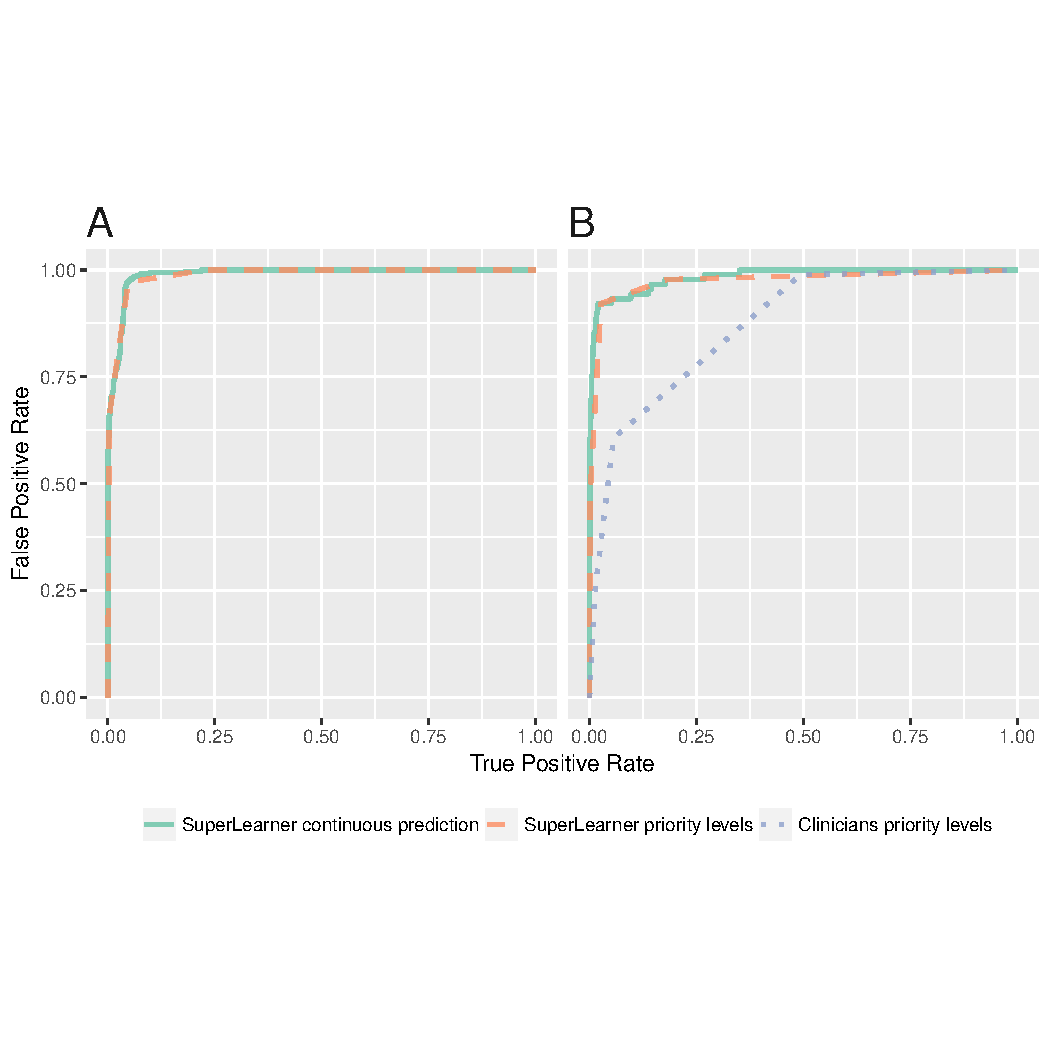
\includegraphics[width=\textwidth]{roc_plot.pdf}
\end{figure}

% **** Calibration plot
\begin{figure}
  \caption{Agreement between the continuous SuperLearner prediction and observed
    all cause 30-day mortality in the training (A) and test (B) samples.}
  \label{fig:calibration_plot}
  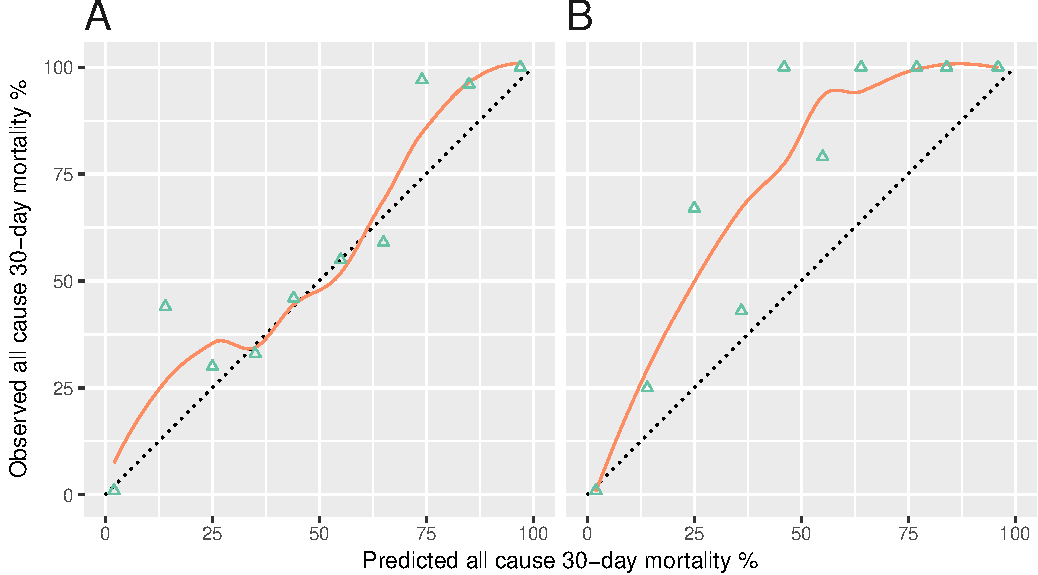
\includegraphics[width=\textwidth]{calibration_plot.pdf}
  \caption*{The straight dotted line indicates perfect agreement. The solid
    orange line is a smoothed association between mean mortality and mean
    predicted mortality across deciles of predicted mortality. The triangles are
    mortality point estimates across the same deciles.}
\end{figure}

% **** Mortality plot
\begin{figure}
  \caption{All cause 30-day mortality across priority levels in the test sample}
  \label{fig:mortality_plot}
  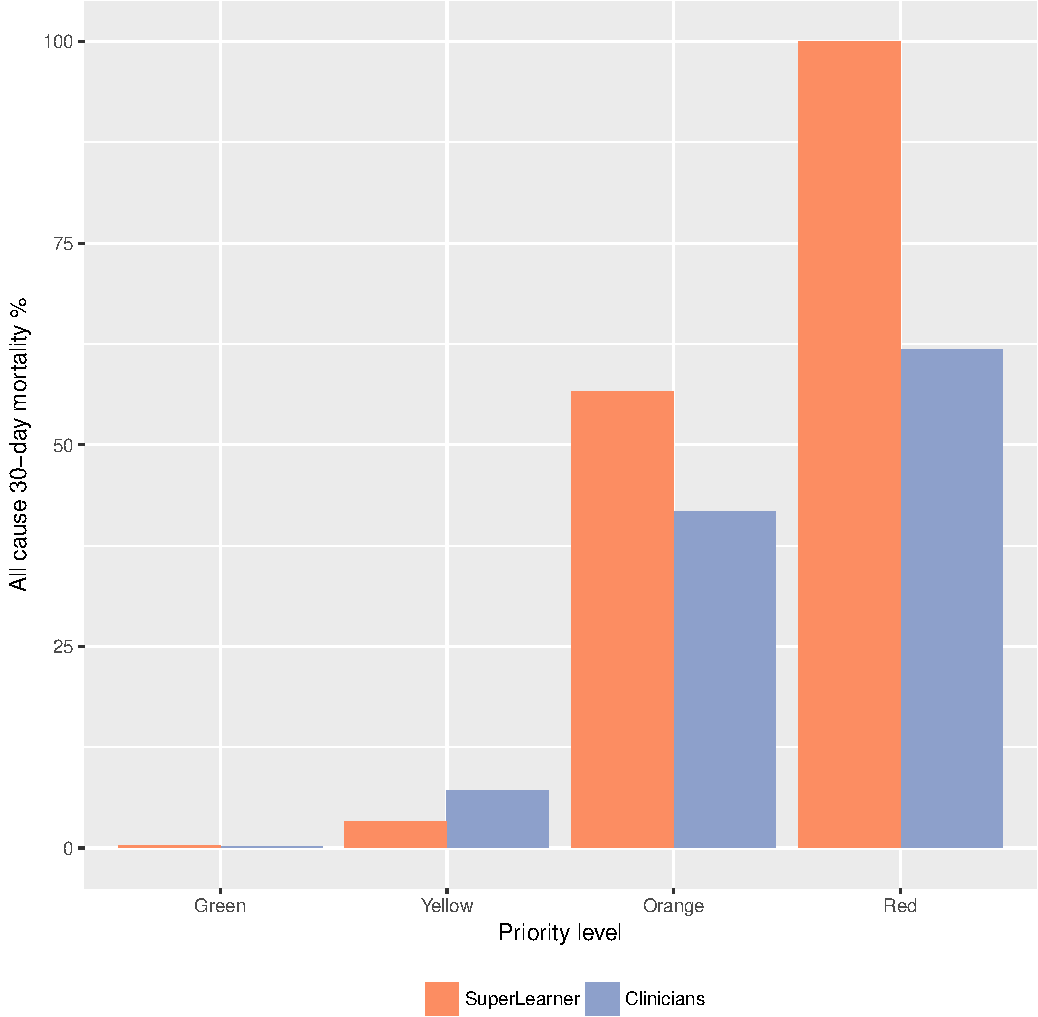
\includegraphics[width=\textwidth]{mortality_plot.pdf}
\end{figure}

% ** Discussion
\section*{Discussion}
Our results indicate that using an ensemble machine learner developed with the
SuperLearner to prioritise among adult trauma patients in the ED is non-inferior
to that of clinician gestalt. In fact, our results suggest that the ensemble
learner is superior to clinician gestalt, both in terms of classification and
discrimination. We have not been able to identify any previous study that has
applied machine learning to prioritise among trauma patients in the ED. Hence,
as far as we know this is the first study of its kind in this area and we hope
that our results can work as benchmarks to which future work can be compared.

Our study was limited by the relatively small sample size. For example, we did
not have enough data to run centre wise analysis, which should be a focus of
future studies. Instead we concentrated on data quality and had dedicated
project officers record all data. This resulted in very low levels of missing
feature data. In contrast, we did have a considerable amount of missing outcome
data, about 20\% of patients were lost to follow up. We handled this missingness
using list wise deletion, aware of the potential bias introduced by this
approach. One alternative would have been to use multiple imputation to replace
missing values, however we had no way of determining the mechanism underlying
the missing outcomes why results based on multiple imputed data might be biased
as well. Further, we did not consider it computionally feasible to combine
multiple imputation and bootstraping for uncertainty estimation. We do however
consider it a strength of our study that the outcome included out of hospital
deaths, when comparably recent research does not \cite{Levin2018, Kunitake2018}.

We used point measurements to train the ensemble learner, meaning that we failed
to account for potential changes in patients' clinical condition between the
time when feature and outcome data were collected. The clinicians were however
also limited to the data available when they decided on a priority level,
although this could have included laboratory or imaging findings from a
transferring health facility. Future research may improve the predictions by
both the ensemble machine learner and clinicians by including data from multiple
time points.

As opposed to the clinicians the ensemble learner was limited by the features
that we defined. In our setting with no or very limited electronic record
keeping it would have been challenging to incorporate for example imaging
data. In settings with more extensive electronic recors this should be more
feasible. Further, the ensemble learner was limited by the techniques included
in its library. We included a mix of MHTM and MMTH learners, for example
logistic regression and random forest. Now, the performance of our ensemble
learner was already very good, but extending the list of features and techniques
available to the learner would likely improve it further.  Also, we used the
default hyperparameter settings for each technique. Future research may improve
the learner's performance by modifying the included learners' hyperparameters.

As stated above there is little research to which our study can be directly
compared. We found that the ensemble learner in general reclassified events to a
higher priority level and non-events to a lower priority level, compared to
clinicians. This is analogous to reduced under and overtriage
respectively. These concepts are used extensively in the trauma
literature. Undertriage refers to for example patients with major trauma not
being transferred to a trauma centre and undertriage to patients with minor
trauma being transferred to a trauma centre. Three studies have used MMTH
learners to limit under and overtriage of trauma patients.  Talbert et
al. applied a tree based learner but found no improvement over standard criteria
\cite{Talbert2007}. More recent research by Follin et al. demonstrated superior
performance of the tree based learner compared to a model based on logistic
regression \cite{Follin2016}. Pearl et al. used neural networks but could not
demonstrate a difference \cite{Pearl2008}. Only Follin report performance
measures that can be compared to our results. Their learner achieved an AUROCC
of 0.82, which is substantially lower than that of our ensemble learner.

In contrast, the literature is replete with studies using MHTM learners to
reduce under and overtriage, or predict trauma mortality \cite{Rehn2011,
  DeMunter2017,VanRein2018}. The performance of these learners vary
substantially, but many studies report AUROCCs that approaches that of our
ensemble learner. For example, Miller et al. and Kunitake et al. achieved
AUROCCs of almost 0.97 and 0.94 with their models based on logistic regression
\cite{Miller2017}. Neither of these studies however approached the problem of
prioritising among trauma patients in the ED, or suggested how the models could
be used to assign patients to different priority levels.

Several steps remain before a system to prioritse among adult trauma patients in
the ED based on our algorithm can and should be implemented. These steps involve
refining the algorithm, comparing it with other commonly used methods to
prioritise patients in the ED, incorporating it into usable software, and
designing an implementation study to assess both its effectiveness and
safety. There are many ways in which the algorithm could be refined but we
regard defining a sequence in which the variables should be measured as the most
important. We think that this sequence should be based on a combination of
individual variable importance and how feasible the variables are to record. We
assume that once this sequence is defined the patients with the most severe
trauma could be identified very quickly using only a small subset of the
variables. Further, our ensemble learner did assign more events to the green
priority level than the clinicians. This should be explored in depth in future
studies.

% Discussion points
% - Improve triage by clinicians
% Mohan D, Farris C, Fischhoff B, Rosengart MR, Angus DC, Yealy DM, et
% al. Efficacy of educational video game versus traditional educational apps at
% improving physician decision making in trauma triage: Randomized controlled
% trial. BMJ. 2017;359(j5416).
% - Physician characteristics associated with good triage
% Mohan D, Barnato AE, Rosengart MR, Farris C, Yealy DM, Switzer GE, et al. Trauma
% triage in the emergency departments of nontrauma centers: An analysis of
% individual physician caseload on triage patterns. J Trauma Acute Care
% Surg. 2013;74(6):1541–7.
% - Paramedic judgement
% Mulholland SA, Gabbe BJ, Cameron P. Is paramedic judgement useful in
% prehospital trauma triage? Injury. 2005;36(11):1298–305.
% - Physicians predict need for lifesaving interventions
% Anazodo AN, Murthi SB, Frank MK, Hu PF, Hartsky L, Imle PC, et al. Assessing
% trauma care provider judgement in the prediction of need for life-saving
% interventions. Injury. 2015;46(5):791–7.

% ** Conclusion
\section*{Conclusion}
An ensemble machine learner developed with the SuperLearner to prioritise among
adult trauma patients in the ED is non-inferior to that of clinician gestalt.

% ** Acknowledgments
\section*{Acknowledgments}
Remains to be written.
% ** Bibliography
\bibliographystyle{unsrt}
\bibliography{bibliography}
% \begin{thebibliography}{10}
% % *** Brohi2017
% \bibitem{Brohi2017}
%   Brohi K, Schreiber M.
%   \newblock {The new survivors and a new era for trauma research.}
%   \newblock PLoS Med. 2017;14(7):3–5.   
% % *** GBD2017
% \bibitem{GBD2017}
%   GBD 2016 Causes of Death Collaborators
%   \newblock {Global, regional, and national age-sex specific mortality for 264
%     causes of death, 1980 – 2016: a systematic analysis for the Global Burden of
%     Disease Study 2016}.
%   \newblock Lancet. 2017 September 16;390:1151–210.
% % *** UN2018
% \bibitem{UN2018}
%   United Nations, Division for Sustainable Development
%   \newblock {Sustainable development goal 3.  Ensure healthy lives and promote
%     well-being for all at all ages}
%   \newblock [Cited 4 May 2018]. Available from: \url{https://sustainabledevelopment.un.org/sdg3}
% % *** Yeboah2014
% \bibitem{Yeboah2014}
%   Yeboah D, Mock C, Karikari P, Agyei-Baffour P, Donkor P, Ebel B.
%   \newblock {Minimizing preventable trauma deaths in a limited-resource setting:
%     A test-case of a multidisciplinary panel review approach at the Komfo Anokye
%     Teaching Hospital in Ghana.}
%   \newblock World J Surg. 2014;38(7):1707–12.
% % *** OReilly2013  
% \bibitem{OReilly2013}
%   O’Reilly D, Mahendran K, West A, Shirley P, Walsh M, Tai N.
%   \newblock {Opportunities for improvement in the management of patients who die
%     from haemorrhage after trauma.}
%   \newblock Br J Surg. 2013;100:749–55.                                             
% % *** Roy2017  
% \bibitem{Roy2017}
%   Roy N, Veetil DK, Khajanchi MU, Kumar V, Solomon H, Kamble J, et al.
%   \newblock {Learning from 2523 trauma deaths in India - opportunities to
%     prevent in-hospital deaths.}
%   \newblock BMC Health Serv Res. 2017;17(142):1–8.
% % *** Fitzgerald2011                                                                  
% % \bibitem{Fitzgerald2011}                                                              
% %   Fitzgerald M, Cameron P, Mackenzie C, Farrow N, Scicluna P, Gocentas R, et al.      
% %   \newblock {Trauma Resuscitation Errors and Computer-Assisted Decision Support}.     
% %   \newblock Arch Surg. 2011;146(2):218–25.                                            
% % *** EAST2010                                                                        
% \bibitem{EAST2010}                                                                    
%   Eastern Association for the Surgery of Trauma (EAST).                               
%   \newblock{Practice Management Guidelines for the Appropriate Triage of the Victim of
%     Trauma.}
%   \newblock EAST. 2010.
% % *** NICE2016
% \bibitem{NICE2016}
%   National Institute for Health and Care Excellence (NICE)
%   \newblock{Major trauma: service delivery}
%   \newblock NICE. 2016.
% % *** Voskens2018
% \bibitem{Voskens2018}
%   Voskens FJ, van Rein EAJ, van der Sluijs R, Houwert RM, Lichtveld RA,
%   Verleisdonk EJ, et al.
%   \newblock{Accuracy of Prehospital Triage in Selecting Severely Injured Trauma
%     Patients.}
%   \newblock  JAMA Surg. 2018 April;153(4):322–7.
% % *** Granstrom2018
% \bibitem{Granstrom2018}
%   Granström A, Strömmer L, Schandl A, Östlund A.
%   \newblock {A criteria-directed protocol for in-hospital triage of trauma
%     patients.}
%   \newblock Eur J Emerg Med. 2018;25(1):25–31.
% % *** ASCOT2014
% \bibitem{ASCOT2014}
%   Committee on Trauma American College of Surgeons.
%   \newblock{Resources for the optimal care of the injured patient.}
%   \newblock{Chicago; 2014.}
% % *** Tignanelli2018
% \bibitem{Tignanelli2018}
%   Tignanelli CJ, Vander Kolk WE, Mikhail JN, Delano MJ, Hemmila MR.
%   \newblock{Noncompliance with American College of Surgeons Committee on Trauma
%     recommended criteria for full trauma team activation is associated with
%     undertriage deaths.}
%   \newblock{J Trauma Acute Care Surg. 2018;84(2):287–94.}
% % *** Benjamin2018
% \bibitem{Benjamin2018}
%   Benjamin ER, Khor D, Cho J, Biswas S, Inaba K, Demetriades D.
%   \newblock{The Age of Undertriage: Current Trauma Triage Criteria Underestimate
%     The Role of Age and Comorbidities in Early Mortality.}
%   \newblock{J Emerg Med. 2018;(April):1–10.}
% % *** VanRein2018
% \bibitem{VanRein2018}
%   van Rein EAJ, van der Sluijs R, Houwert RM, Gunning AC, Lichtveld RA, Leenen LPH, et al.
%   \newblock {Effectiveness of prehospital trauma triage systems in selecting
%     severely injured patients: Is comparative analysis possible?}
%   \newblock Am J Emerg Med. 2018.
% % *** SATG2012
% \bibitem{SATG2012}
%   South African Triage Group.
%   \newblock{The South African Triage Scale Training Manual 2012.}
%   \newblock{Western Cape Government. 2012.}
% % *** ESI2012
% \bibitem{ESI2012}
%   Agency for Healthcare Research and Quality.
%   \newblock{Emergency Severity Index (ESI). A Triage Tool for Emergency Department Care.}
%   \newblock{U.S. Department of Health \& Human Services. 2012; Version 4.}
% % *** Baker2013
% \bibitem{Baker2013}
%   Baker T, Lugazia E, Eriksen J, Mwafongo V, Irestedt L, Konrad D.
%   \newblock{Emergency and critical care services in Tanzania.}
%   \newblock{BMC Health Serv Res. 2013;13(140).}
% % *** Choi2017
% \bibitem{Choi2017}
%   Choi SJ, Oh MY, Kim NR, Jung YJ, Ro YS, Shin S Do.
%   \newblock{Comparison of trauma care systems in Asian countries: A systematic literature review.}
%   \newblock{Emerg Med Australas. 2017;29(June):697–711. }
% % *** Beam2018
% \bibitem{Beam2018}
%   Beam AL, Kohane IS.
%   \newblock{Big Data and Machine Learning in Health Care.}
%   \newblock{Jama. 2018 March 12;E1–2.}
% % *** Nevin2018
% \bibitem{Nevin2018}
%   Nevin L.
%   \newblock{Human Intelligence \& Artificial Intelligence in Medicine: A day with
%     the Stanford Presence Center.}
%   \newblock{PLOS Blogs. 2018 [cited 2018 May 5]. Available from:
%     http://blogs.plos.org/speakingofmedicine/2018/04/24/human-intelligence-artificial-intelligence-in-medicine-a-day-with-the-stanford-presence-center/}
% % *** Liu2017
% \bibitem{Liu2017}
%   Liu NT, Salinas J.
%   \newblock{Machine Learning for Predicting Outcomes in Trauma.}
%   \newblock{Shock. 2017;48(5):504–10.}
% % *** Talbert2007
% \bibitem{Talbert2007}
%   Talbert S, Talbert DA.
%   \newblock{A comparison of a decision tree induction algorithm with the ACS guidelines for trauma triage.}
%   \newblock{AMIA Annu Symp Proc. 2007;1127.}
% % *** Pearl2008
% \bibitem{Pearl2008}
%   Pearl A, Bar-Or R, Bar-Or D.
%   \newblock{An artificial neural network derived trauma outcome prediction score as an aid to triage for non-clinicians.}
%   \newblock{Stud Heal Technol Informatics. 2008;136:253–8.}
% % *** Scerbo2014
% \bibitem{Scerbo2014}
%   Scerbo M, Radhakrishnan H, Cotton B, Dua A, Del Junco D, Wade C, et al.
%   \newblock{Prehospital triage of trauma patients using the Random Forest
%     computer algorithm.}
%   \newblock{J Surg Res. 2014;187(2):371–6.}
% % *** Follin2016
% \bibitem{Follin2016}
%   Follin A, Jacqmin S, Chhor V, Bellenfant F, Robin S, Guinvarc’h A, et al.
%   \newblock{Tree-based algorithm for prehospital triage of polytrauma
%     patients.}
%   \newblock{Injury. 2016;47(7):1555–61.}
% % *** Levin2018
% \bibitem{Levin2018}
%   Levin S, Toerper M, Hamrock E, Hinson JS, Barnes S, Gardner H, et al.
%   \newblock{Machine-Learning-Based Electronic Triage More Accurately
%     Differentiates Patients With Respect to Clinical Outcomes Compared With the
%     Emergency Severity Index.}
%   \newblock{Ann Emerg Med. 2018;71(5):565–574.e2.}
% % *** WHOICD
% \bibitem{WHOICD}
%   World Health Organization.
%   \newblock{ICD-10 Interactive Self Learning Tool.}
%   \newblock{WHO [cited 2018 May 7]. Available from: http://apps.who.int/classifications/apps/icd/icd10training/}
% % *** GCSAID
% \bibitem{GCSAID}
%   glasgowcomascale.org.
%   \newblock{GLASGOW COMA SCALE: Do it this way.}
%   \newblock{glasgowcomascale.org [cited 2018 May 7]. Available from: http://www.glasgowcomascale.org/downloads/GCS-Assessment-Aid-English.pdf?v=3}
% % *** Kristiansen2010
% % \bibitem{Kristiansen2010}
% %   Kristiansen T, Søreide K, Ringdal KG, Rehn M, Krüger AJ, Reite A, et al.
% %   \newblock {Trauma systems and early management of severe injuries in
% %     Scandinavia: Review of the current state.}.
% %   \newblock  Injury. 2010;41(5):444–52. 
% % *** Collins2015
% % \bibitem{Collins2015}
% %   Collins GS, Reitsma JB, Altman DG, Moons KGM.
% %   \newblock {Transparent reporting of a multivariable prediction model for
% %     individual prognosis or diagnosis (TRIPOD): The TRIPOD Statement}.
% %   \newblock BMC Med. 2015;13(1).
% % *** Rehn2011
% \bibitem{Rehn2011}
%   Rehn M, Perel P, Blackhall K, Lossius HM.
%   \newblock {Prognostic models for the early care of trauma patients: a
%     systematic review.}.
%   \newblock Scand J Trauma Resusc Emerg Med. 2011;19(17).
% % *** R
% \bibitem{R}
%   R Core Team
%   \newblock {R: A language and environment for statistical computing.}
%   \newblock {R Foundation for Statistical Computing, Vienna,
%     Austria. 2017. Available from https://www.R-project.org/.}
% % *** SuperLearner
% \bibitem{SuperLearner}
%   Polley E, LeDell E, Kennedy C, van der Laan M.
%   \newblock {SuperLearner: Super Learner Prediction.}
%   \newblock {R package version 2.0-23. 2018. Available from:
%     https://CRAN.R-project.org/package=SuperLearner}
% % *** Example
% % \bibitem{bib3}
% % Magwire MM, Bayer F, Webster CL, Cao C, Jiggins FM.
% % \newblock {{S}uccessive increases in the resistance of {D}rosophila to viral
% %   infection through a transposon insertion followed by a {D}uplication}.
% %   \newblock PLoS Genet. 2011 Oct;7(10):e1002337.
% % *** End bibliography
% \end{thebibliography}
% ** End
\end{document}
